	\paragraph{QuizziPedia::Front-End::Directives::BreadBarDirective}
		
		\label{QuizziPedia::Front-End::Directives::BreadBarDirective}
		
		\begin{figure}[ht]
			\centering
			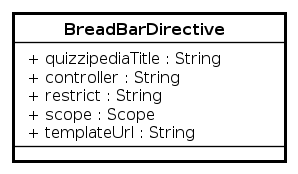
\includegraphics[scale=0.80,keepaspectratio]{UML/Classi/Front-End/QuizziPedia_Front-end_Directives_BreadBarDirective.png}
			\caption{QuizziPedia::Front-End::Directives::BreadBarDirective}
		\end{figure} \FloatBarrier
		
		\begin{itemize}
			\item \textbf{Descrizione}: rappresenta il menù, presente in ogni pagina dell'applicazione,
generato in base agli oggetti passati nello \$scope isolato. Fornisce un
pulsante per ogni oggetto ricevuto come parametro, ogni pulsante viene
rappresentato con un'icona e con un testo. Al click di un pulsante viene
invocata la funzione ad esso associata;
			\item \textbf{Utilizzo}: viene utilizzato per facilitare la navigazione all'interno dell'applicazione;
			\item \textbf{Relazioni con altre classi}: 
			\begin{itemize}
				\item \textbf{IN \texttt{Index}}: contenitore generale dell'applicazione;
				\item \textbf{IN \texttt{SearchDirective}}: \textit{directive\ped{G}} che permette di effettuare la ricerca di utenti e questionari;
				\item \textbf{IN \texttt{LoginBarDirective}}: \textit{directive\ped{G}} contenente il componente che permette di effettuare il redirect alla pagina di login;
				\item \textbf{IN \texttt{SignUpBarDirective}}: \textit{directive\ped{G}} contenente il componente che permette di effettuare il redirect alla pagina di registrazione;
				\item \textbf{IN \texttt{UserBarDirective}}: \textit{directive\ped{G}} contenente il componente che permette di effettuare il redirect alla pagina di visualizzazione del profilo utente personale;
				\item \textbf{IN \texttt{ProfileManagementBarDirective}}: \textit{directive\ped{G}} contenente il componente che permette di effettuare il redirect alla pagina di gestione del profilo;
				\item \textbf{IN \texttt{QuestionsManagementBarDirective}}: \textit{directive\ped{G}} contenente il componente che permette di effettuare il redirect alla pagina di gestione delle domande;
				\item \textbf{IN \texttt{LogoutBarDirective}}: \textit{directive\ped{G}} contenente il componente che permette di effettuare il logout;
				\item \textbf{IN \texttt{QuestionnaireManagementBarDirective}}: \textit{directive\ped{G}} contenente il componente che permette di effettuare il redirect alla pagina di gestione dei questionari.;
			\end{itemize}
			\item \textbf{Attributi}:
			\begin{itemize}
		\item \texttt{+ quizzipediaTitle: String} \\ Attributo che viene utilizzato per visualizzare la giusta traduzione della \textit{label\ped{G}} per il titolo e la descrizione dell'applicazione;
		\item \texttt{+ controller: String} \\ Stringa contenente il nome del \textit{controller\ped{G}} della direttiva;
		\item \texttt{+ restrict: String} \\ Stringa che permette di definire le modalità di inserimento della direttiva all'interno della pagina;
		\item \texttt{+ scope: Scope}: oggetto scope interno della direttiva, contiene le funzionalità per gestire i dati presenti all'interno;
		\item \texttt{+ templateUrl: String} \\ Stringa contenente il percorso del file \textit{HTML\ped{G}} che contiene la direttive.
	\end{itemize}
		\end{itemize}